\documentclass[12pt,twoside]{article}

\newcommand{\reporttitle}{M111: Big Data Management}
\newcommand{\reportauthor}{Michael Darmanis\textsuperscript{*}}
\newcommand{\reporttype}{Project}
\newcommand{\sid}{7115152200004}

% include files that load packages and define macros
\input{includes} % various packages needed for maths etc.
\input{notation} % short-hand notation and macros


%%%%%%%%%%%%%%%%%%%%%%%%%%%%

\begin{document}
% front page
% Last modification: 2016-09-29 (Marc Deisenroth)
\begin{titlepage}

\newcommand{\HRule}{\rule{\linewidth}{0.5mm}} % Defines a new command for the horizontal lines, change thickness here


%----------------------------------------------------------------------------------------
%	LOGO SECTION
%----------------------------------------------------------------------------------------

\includegraphics[width=7cm]{./figures/NKUA-logo}\\[0.5cm]

\begin{center} % Center remainder of the page

%----------------------------------------------------------------------------------------
%	HEADING SECTIONS
%----------------------------------------------------------------------------------------
\textsc{\LARGE \reporttype}\\[1.5cm] 
\textsc{\Large National and Kapodistrian University of Athens}\\[0.5cm] 
\textsc{\large Faculty of Informatics and Telecommunications }\\[0.5cm]
% \textsc{\large MSc. Data Science and Information Technologies}\\[0.5cm]
%----------------------------------------------------------------------------------------
%	TITLE SECTION
%----------------------------------------------------------------------------------------

\HRule \\[0.4cm]
{ \huge \bfseries \reporttitle}\\ % Title of your document
\HRule \\[1.5cm]
\end{center}
%----------------------------------------------------------------------------------------
%	AUTHOR SECTION
%----------------------------------------------------------------------------------------

%\begin{minipage}{0.4\hsize}
\begin{flushleft} \large
\textit{Author:}\\
\reportauthor~(SID: \sid)% Your name
\end{flushleft}
\vspace{2cm}
\makeatletter
Date: \@date\\
\textsuperscript{*}\href{mailto:mdarm@di.uoa.gr}{mdarm@di.uoa.gr}

\vfill % Fill the rest of the page with whitespace



\makeatother


\end{titlepage}



%%%%%%%%%%%%%%%%%%%%%%%%%%%% Main document
\section{Introduction}

\subsection{}
For creating a \texttt{files} directory in the HDFS, the following command was used
\mint{bash}|hadoop fs -mkdir -p ~/files|
\noindent and to populate it with the project's \texttt{.csv} files
\mint{bash}|hadoop fs -put *.csv ~/files .|
\noindent Since the only \texttt{.csv} files populating the working directory were the project's ones, it was fairly easy to fetch all of them using \texttt{*.csv}.
Fig.~\ref{fig:files} shows a print-screen of the \texttt{.csv} files lying within the created \texttt{files} directory.

\begin{figure}[htbp]
    \centering
    \includegraphics[width=\textwidth]{./figures/files.png}
    \caption{HDFS directory containing the project's datasets in \texttt{.csv} format.}
    \label{fig:files}
\end{figure}

The same files were then saved in \texttt{.parquet} format, using Snip.~\ref{code:files}, as can be seen in the print-screen of Fig~\ref{fig:files-all}.

\begin{figure}[htbp]
    \centering
    \includegraphics[width=\textwidth]{./figures/files-all.png}
    \caption{HDFS directory containing the project's datasets in both \texttt{.csv} and \texttt{.parquet} formats.}
    \label{fig:files-all}
\end{figure}

\section{Basics}

\subsection{Repartition and Broadcast Joins}

\begin{figure}[htb]
    \centering
    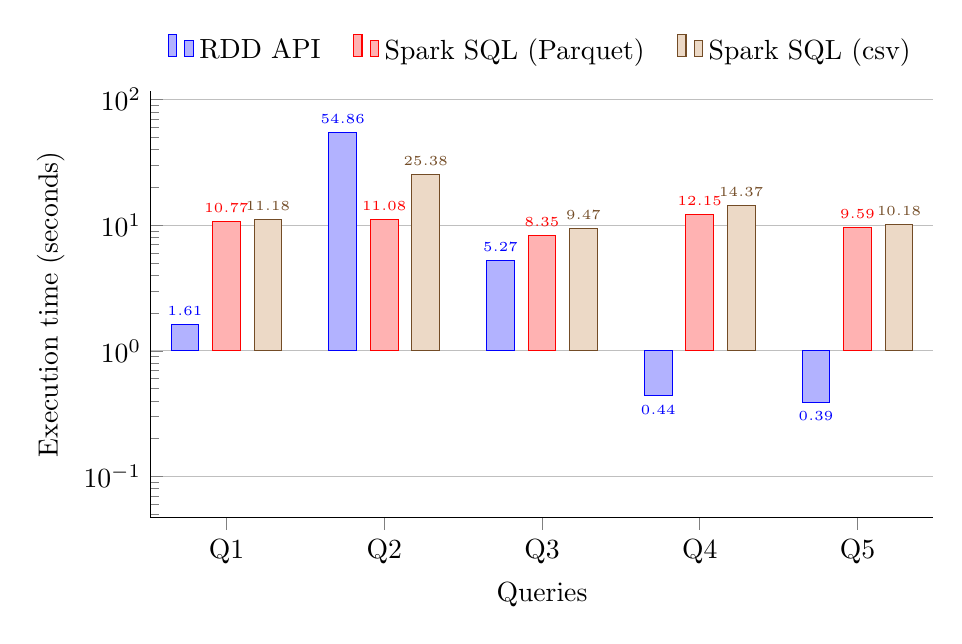
\begin{tikzpicture}
\begin{axis}[
    ybar=5pt,
    enlargelimits=0.12,
    bar width=10pt,
    ylabel={Execution time (seconds)},
    xlabel={Queries},
    width=0.95\textwidth,
    height=7cm,
    symbolic x coords={Q1,Q2,Q3,Q4,Q5},
    xtick=data,
    ymode=log,
    ymin=0.1,
    ymajorgrids=true,
    axis x line* = bottom,
    axis y line* = left,
    legend style={cells={anchor=west}, draw=none},
    legend style={at={(0.5,1.15)}, anchor=north,legend columns=-1},
    legend columns=-1,
    point meta=explicit symbolic,
    nodes near coords=\pgfmathprintnumber{\pgfplotspointmeta},
    visualization depends on={y<0.2?0:1 \as \myshift},
    every node near coord/.append style={font=\tiny, anchor=north, yshift=(\myshift*10pt)},
    ]
\addplot table [meta=Y] {
  X Y
  Q1  1.61
  Q2 54.86
  Q3  5.27
  Q4  0.44
  Q5  0.39
};

\addplot table [meta=Y] {
  X Y
  Q1 10.77
  Q2 11.08
  Q3  8.35
  Q4 12.15
  Q5  9.59
};

\addplot table [meta=Y] {
  X Y
  Q1 11.18
  Q2 25.38
  Q3  9.47
  Q4 14.37
  Q5 10.18
};

\legend{RDD API\hphantom{xz}, Spark SQL (Parquet)\hphantom{xz} , Spark SQL (csv) }
\end{axis}
\end{tikzpicture}
    \caption{Caption}
    \label{fig:enter-label}
\end{figure}

\subsection{Tweaking the Catalyst Optimiser}

\begin{figure}[htb]
    \centering
    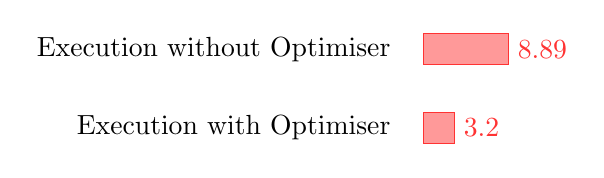
\begin{tikzpicture}
  \begin{axis}[,
    xbar,
    y axis line style = { opacity = 0 },
    axis x line       = none,
    tickwidth         = 0pt,
    ytick             = data,
    enlarge y limits  = 0.2,
    enlarge x limits  = 1,
    y = 1cm,
    width=0.3\textwidth,
    bar width=4mm,
    symbolic y coords = {Execution with Optimiser, Execution without Optimiser},
    nodes near coords,
  ]
  \addplot[red!80, fill=red!40] coordinates { (3.20,Execution with Optimiser) (8.89,Execution without Optimiser)};
  \end{axis}
\end{tikzpicture}
    \caption{Execution time, for a particular query, with and without Spark's SQL Optimiser.}
    \label{fig:enter-label1}
\end{figure}

Without Optimization (Sort Merge Join):

\begin{minted}{bash}
== Physical Plan ==
*(6) SortMergeJoin [mv_id#8], [mv_id#1], Inner
\end{minted}

\noindent This is a Sort Merge Join, which is an operation where two dataframes are joined by sorting the data and then merging the sorted data. This type of join is used when the data is too large to fit into memory for a Broadcast Join.

The stages of this join operation involve filtering data where mv\textunderscore id is not null, limiting the result set to 100, then sorting the data and performing the join operation. The SortMergeJoin operation requires that both sides of the join have been partitioned and sorted by the join key (mv\textunderscore id in this case). Hence, there are additional Sort and Exchange operations before the join.

\begin{minted}{bash}
+- *(2) GlobalLimit 100
+- Exchange SinglePartition
+- *(1) LocalLimit 100
\end{minted}

\noindent These operations represent the limit that is applied to the "movie\textunderscore genres" table (the query limits the result set to 100). The GlobalLimit means that the limit is applied across the entire dataset, not just per partition.

The time taken for the entire operation is 13.2132 seconds.

With Optimization (Broadcast Hash Join):

\begin{minted}{bash}
== Physical Plan ==
*(3) BroadcastHashJoin [mv_id#8], [mv_id#1], Inner, BuildLeft
\end{minted}

\noindent This is a Broadcast Hash Join, which is a type of join operation where the smaller DataFrame is broadcast to all the nodes containing partitions of the larger DataFrame for comparison and join operations. This type of join can be significantly faster than a sort-merge join because it doesn't require the data to be sorted first, and it can be done entirely in memory if the smaller DataFrame is small enough.

\begin{minted}[breaklines, breakafter=d]{bash}
:- BroadcastExchange HashedRelationBroadcastMode(List(cast(input[0, int, false] as bigint)
\end{minted}

\noindent The BroadcastExchange operation represents broadcasting the smaller DataFrame to the worker nodes. The broadcasting operation will transform the DataFrame into a more efficient data structure (a hash table) to speed up the subsequent join operation.

The time taken for the entire operation is 3.7529 seconds, which is significantly faster than the time taken when the optimization is not enabled. The optimizer has chosen a more efficient join strategy (broadcast hash join instead of sort merge join) based on the size of the data and the nature of the operation, which leads to a faster execution time.

Overall, the difference between these two execution plans demonstrates the power and importance of the Spark Catalyst optimizer in efficiently executing Spark jobs. It can make smart decisions, such as using a BroadcastHashJoin instead of a SortMergeJoin, which significantly improves performance.

\section{Code Snippets}
\begin{code}
\captionof{listing}{\texttt{csv\textunderscore to\textunderscore parquet.py}}
\label{code:files}
\inputminted[breaklines, breakafter=d, linenos, frame=single]{python}{./code/csv_to_parquet.py}
\end{code}


\newpage
\pagestyle{empty}
% If you do want an image in the colophon:
\begin{figure}
  \vspace{50pt}
  \centering
  \includegraphics[width=0.51\textwidth]{./figures/colophon}
\end{figure}

% If you don't want an image in the colophon:
% \vspace*{200pt}

\begin{center}
\parbox{200pt}{\lettrine[lines=3,slope=-2pt,nindent=-4pt]{\textcolor{uni-color}{T}}{his coursework was typeset} using LaTeX, originally developed by Leslie Lamport and based on Donald Knuth's TeX. The body text is set in 12 point kpfonts, a revival of URW Palladio typeface. The above illustration, ``Science Experiment 02'', was created by Ben Schlitter and released under \href{http://creativecommons.org/licenses/by-nc-nd/3.0/}{\textsc{cc by-nc-nd 3.0}}. A template that can be used to format coursework with this look and feel has been released under the permissive \href{http://creativecommons.org/licenses/by-nc-nd/4.0/}{\textsc{cc by-nc-nd 4.0}} license, and can be found online at \href{https://cs.overleaf.com/latex/templates/maths-coursework-template/kbyhcwmjdtpf}{https://cs.overleaf.com/latex/}.}
\end{center}

\end{document}
%%% Local Variables: 
%%% mode: latex
%%% TeX-master: t
%%% End: